\chapter{Background\label{cha:chapter2}}

\hspace*{1em}This chapter provides the theoretical and contextual background 
necessary to understand the key concepts and methodologies 
that form the foundation of this thesis.
The first section introduces the fundamentals of deep NNs,
which serve as a basis for the discussion.
The next section broadens the perspective by exploring
the concept of quantization,
followed by the final section that explains common techniques of \textit{learned quantization},
as well as the trade-offs and challenges they present.

% ------------------------------------------------------------
% ----------------------- deeplearning ----------------------- 
% ------------------------------------------------------------
\section{Fundamentals of Deep Learning}
\label{sec:deeplearning}
\hspace*{1em}This section introduces the fundamental concepts of deep learning, 
beginning with the most basic NN architecture components in \cref{subsec:denseconvolutional} and progressing to loss functions with regularization in \cref{subsec:lossregularization}. 
The concepts of the forward-pass and back-propagation will be explained in the last \cref{subsec:forwardback}.

% -------------------- denseconvolutional --------------------
\subsection{Dense and Convolutional Layers}
\label{subsec:denseconvolutional}
\hspace*{1em}
NNs can be considered a mathematical abstraction 
inspired by the structure and function of biological neural systems. 
At their core, they process inputs, transform them through intermediate or \textit{hidden layers} of computation, 
and produce outputs.
These hidden layers, which typically consist of interconnected
neurons, are where the magic
 — or the transformation of data — happens. In its simplest form, 
 within the classic \textit{Multilayer Perceptron} (MLP) model,
 each hidden layer neuron performs a weighted operation:

\[
\textit{output} = f(w \cdot \textit{input} + b)
\]

\begin{itemize}
  \item \( input \in \mathbb{R}^d \) refers to the outputs from the previous layer (or the initial data from input nodes) that are fed into a specific neuron in the hidden layer.
  \item \( w \in \mathbb{R}^d \) (weights) is a vector of parameters associated with that specific neuron, defining the importance of each input received by this neuron. 
  \item \( b \in \mathbb{R} \) (bias) is an additional scalar parameter specific to the neuron, which shifts the result of the weighted sum, allowing for more flexibility.
  \item \( f(\cdot): \mathbb{R} \to \mathbb{R} \) is the \textit{activation function}, a nonlinear function applied to the weighted sum of inputs and bias in that specific neuron, allowing for more complexity.
  \item \( output \in \mathbb{R} \) is the result produced by the neuron, which will then be passed on to the next hidden layer (or to the final output layer).
\end{itemize}

Hidden layers where each neuron is connected to every neuron in the previous layer 
and every neuron in the next layer are called \textit{dense layers}.
The \textit{weight matrix} (\( W\)), which combines the weight vectors of all neurons in a dense layer,
grows linearly with each added neuron or input node, 
embodying the interconnectedness of such layers
 
\begin{figure}[t!]
  \centering
  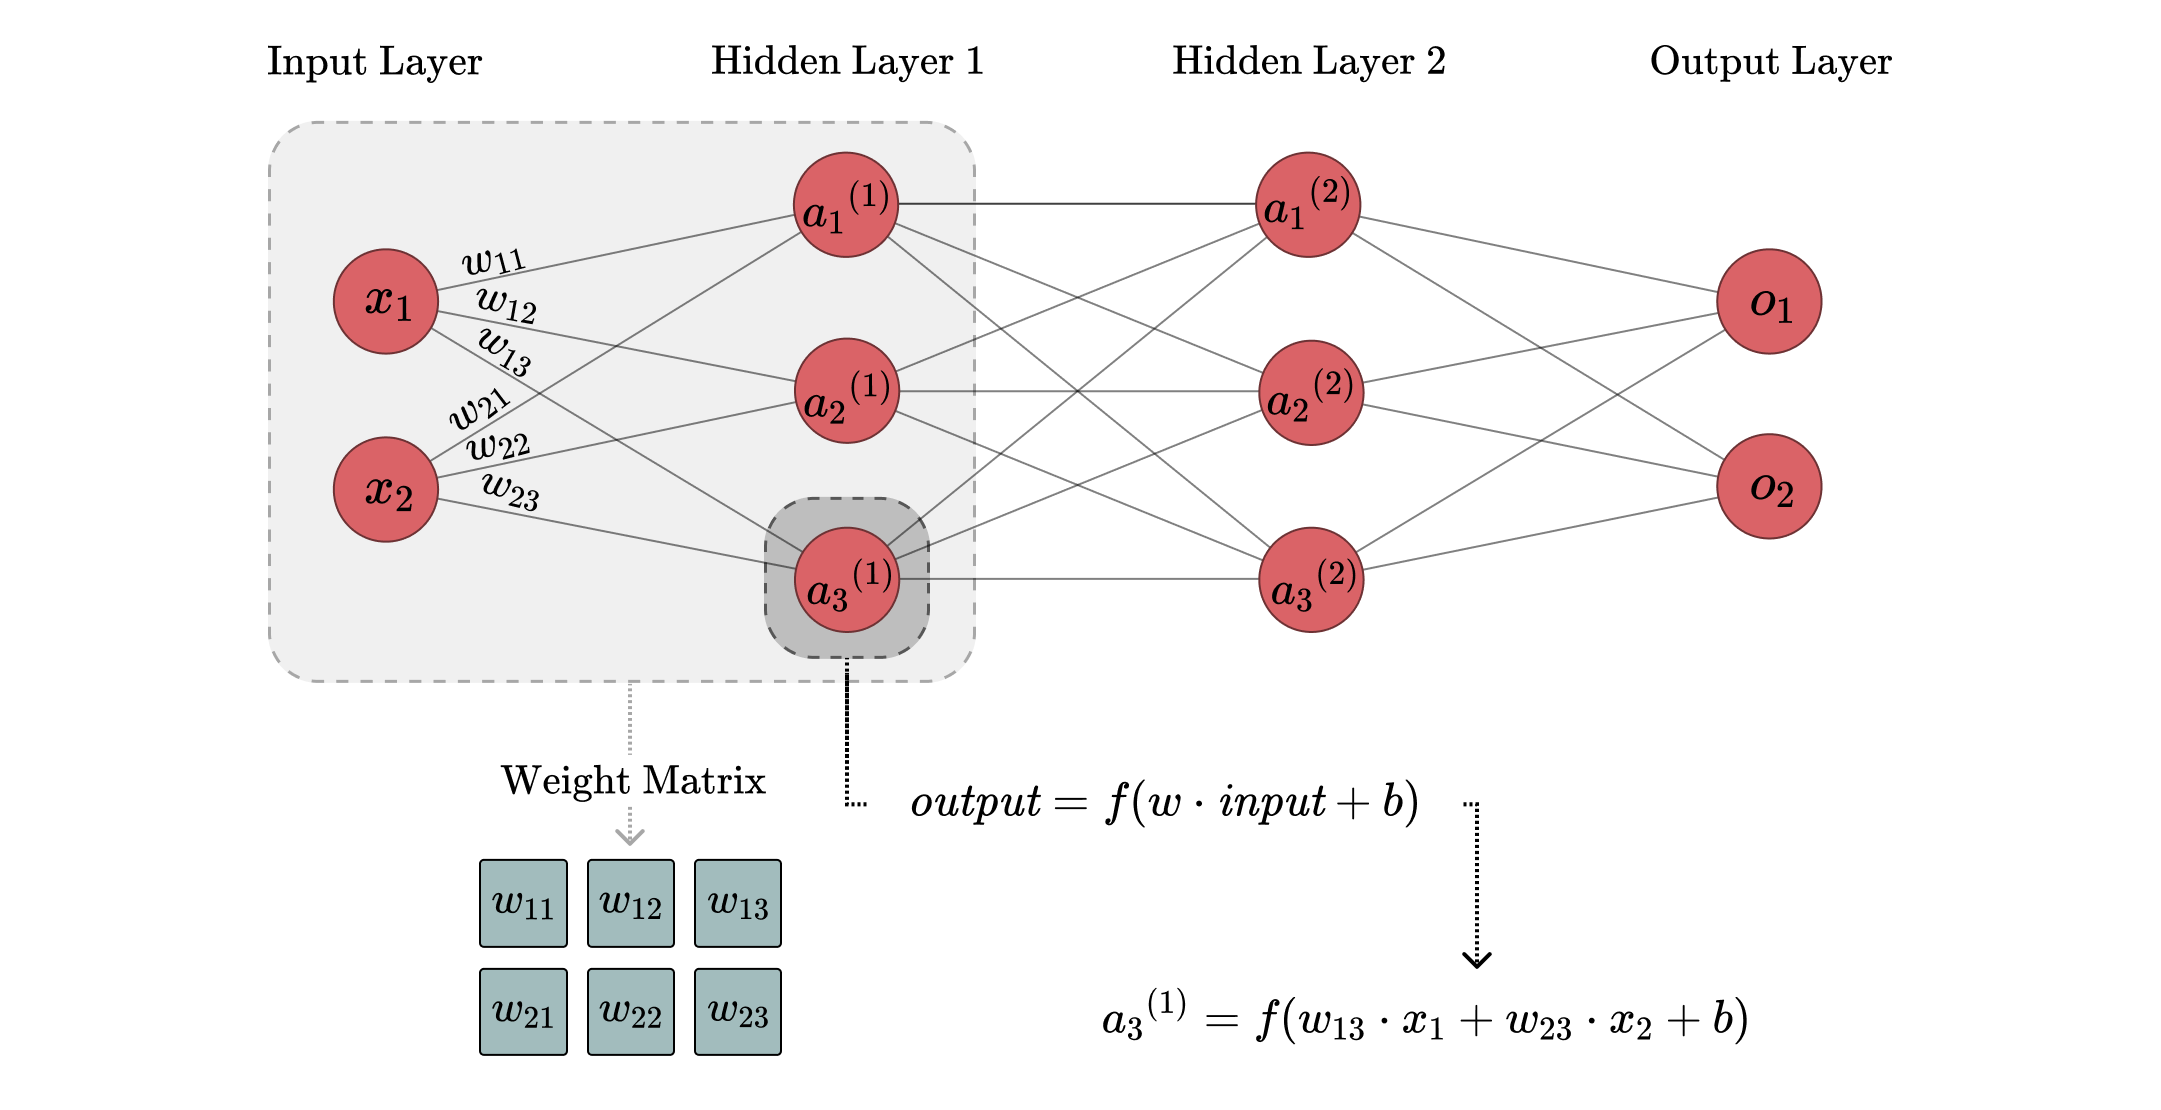
\includegraphics[width=14cm]{dense_layer}
  \caption{An example of an NN with two hidden dense layers, showing the connections between neurons in adjacent layers.}
  \label{fig:dense_layer}
\end{figure}

This interconnected structure introduces the inherent redundancy, or — in other words — the over-parameterization of NNs \cite{gholami2021survey}.
It is particularly true in models with a large number of neurons, 
where \( W \) results in a vast number of parameters, which do not contribute to the model accuracy equally \cite{hubara2016qnn}.

\begin{figure}[b!]
  \centering
  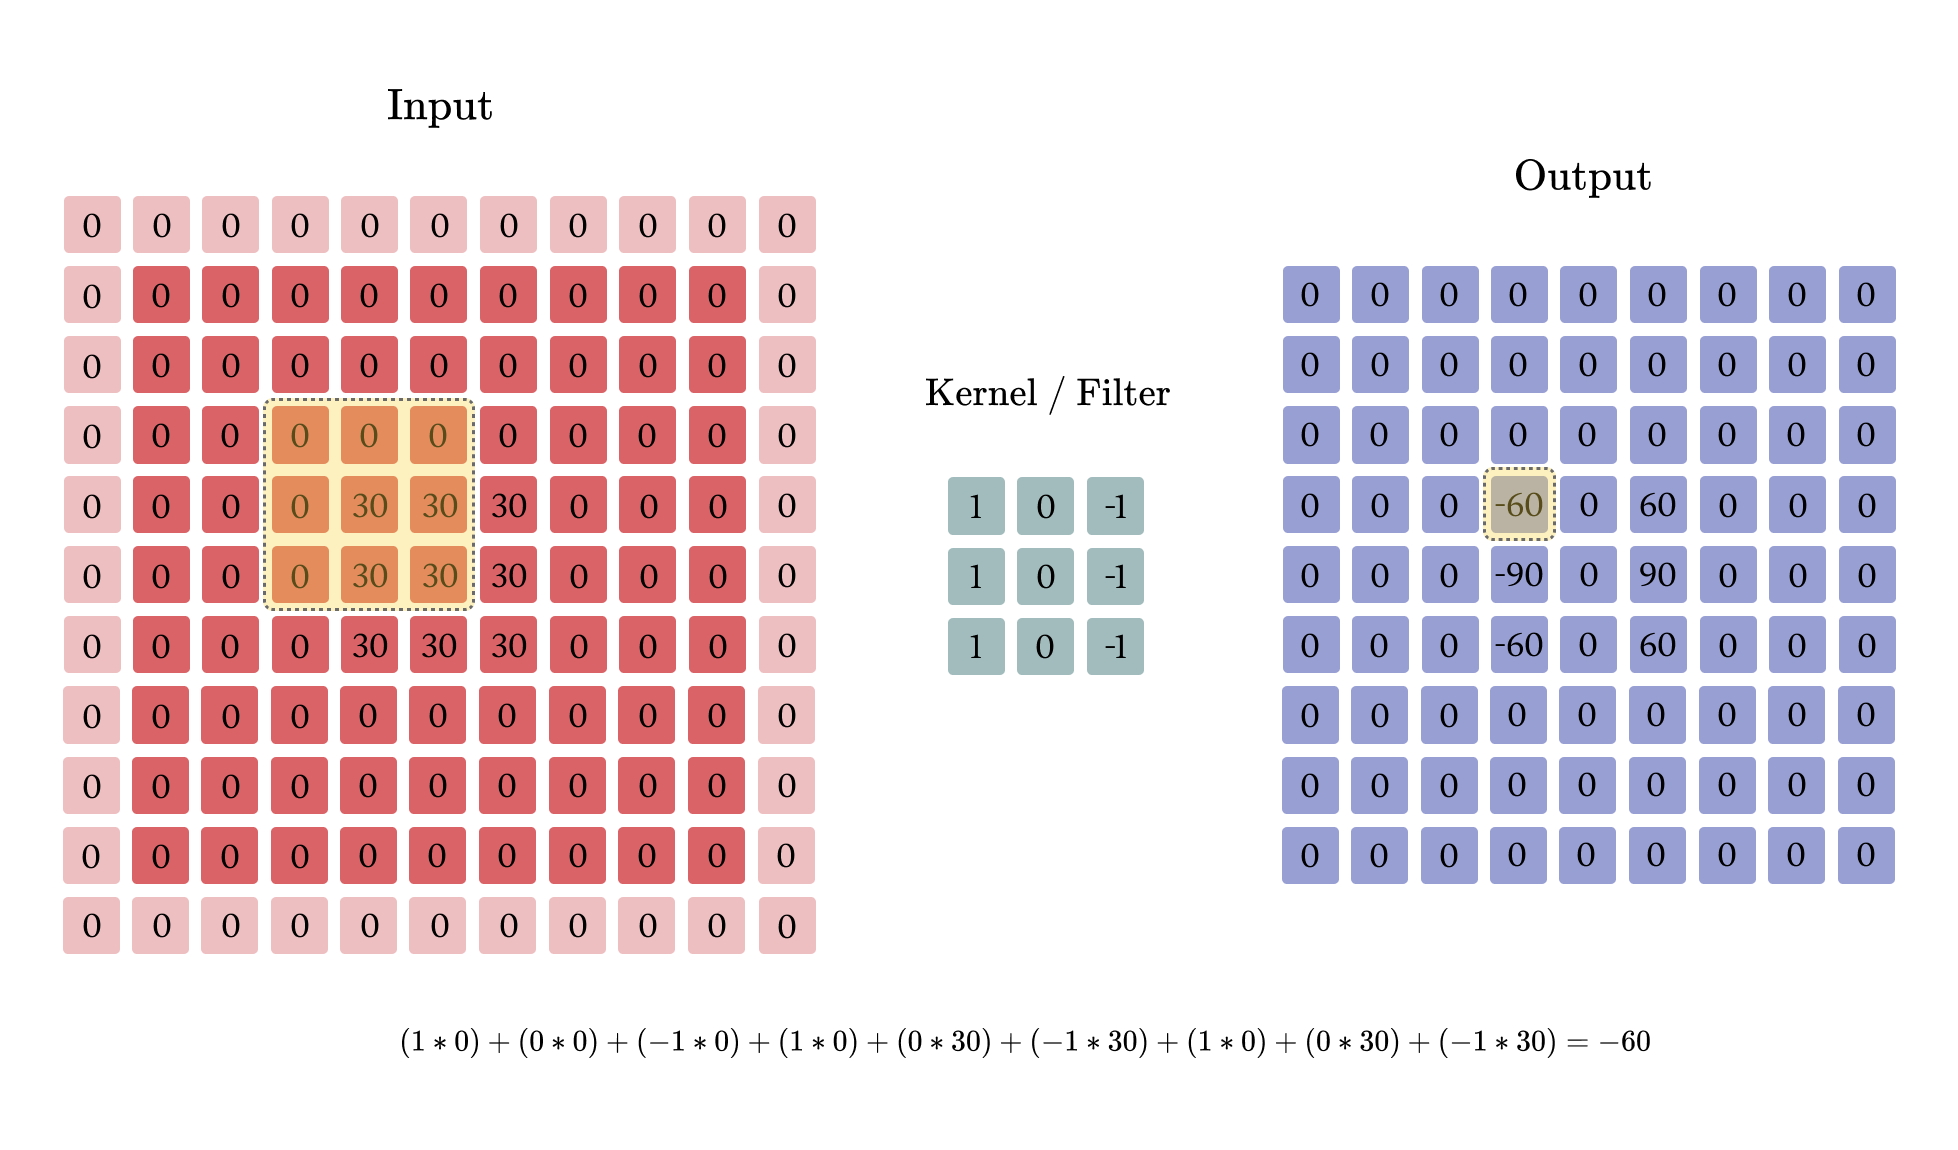
\includegraphics[width=14cm]{convolution}
  \caption{A 3×3 kernel sliding over a padded input matrix to compute the output feature map.}
  \label{fig:convolution}
\end{figure}

\textit{Convolutional layers} are another type of hidden layers 
that involve a \textit{convolution} operation on the input. Intuitively, a standard convolution is 
a process of sliding a small grid, or \textit{kernel}, over an input to find patterns. \cref{fig:convolution}, for example, shows 
the application of the Sobel kernel that detects edges on the input image.
For multi-channeled inputs, like RGB images, the convolution operation uses a multi-channeled kernel, as shown in \cref{fig:convolution_multiple_channels}, 
producing a single-channeled feature map that combines weighted contributions from all input channels. 
A convolutional layer includes multiple such kernels, generating feature maps equal to the number of kernels.
After the convolution operation generates the feature maps, a bias term is added to each map, 
and the activation function is applied element-wise.
\begin{figure}[b!]
  \centering
  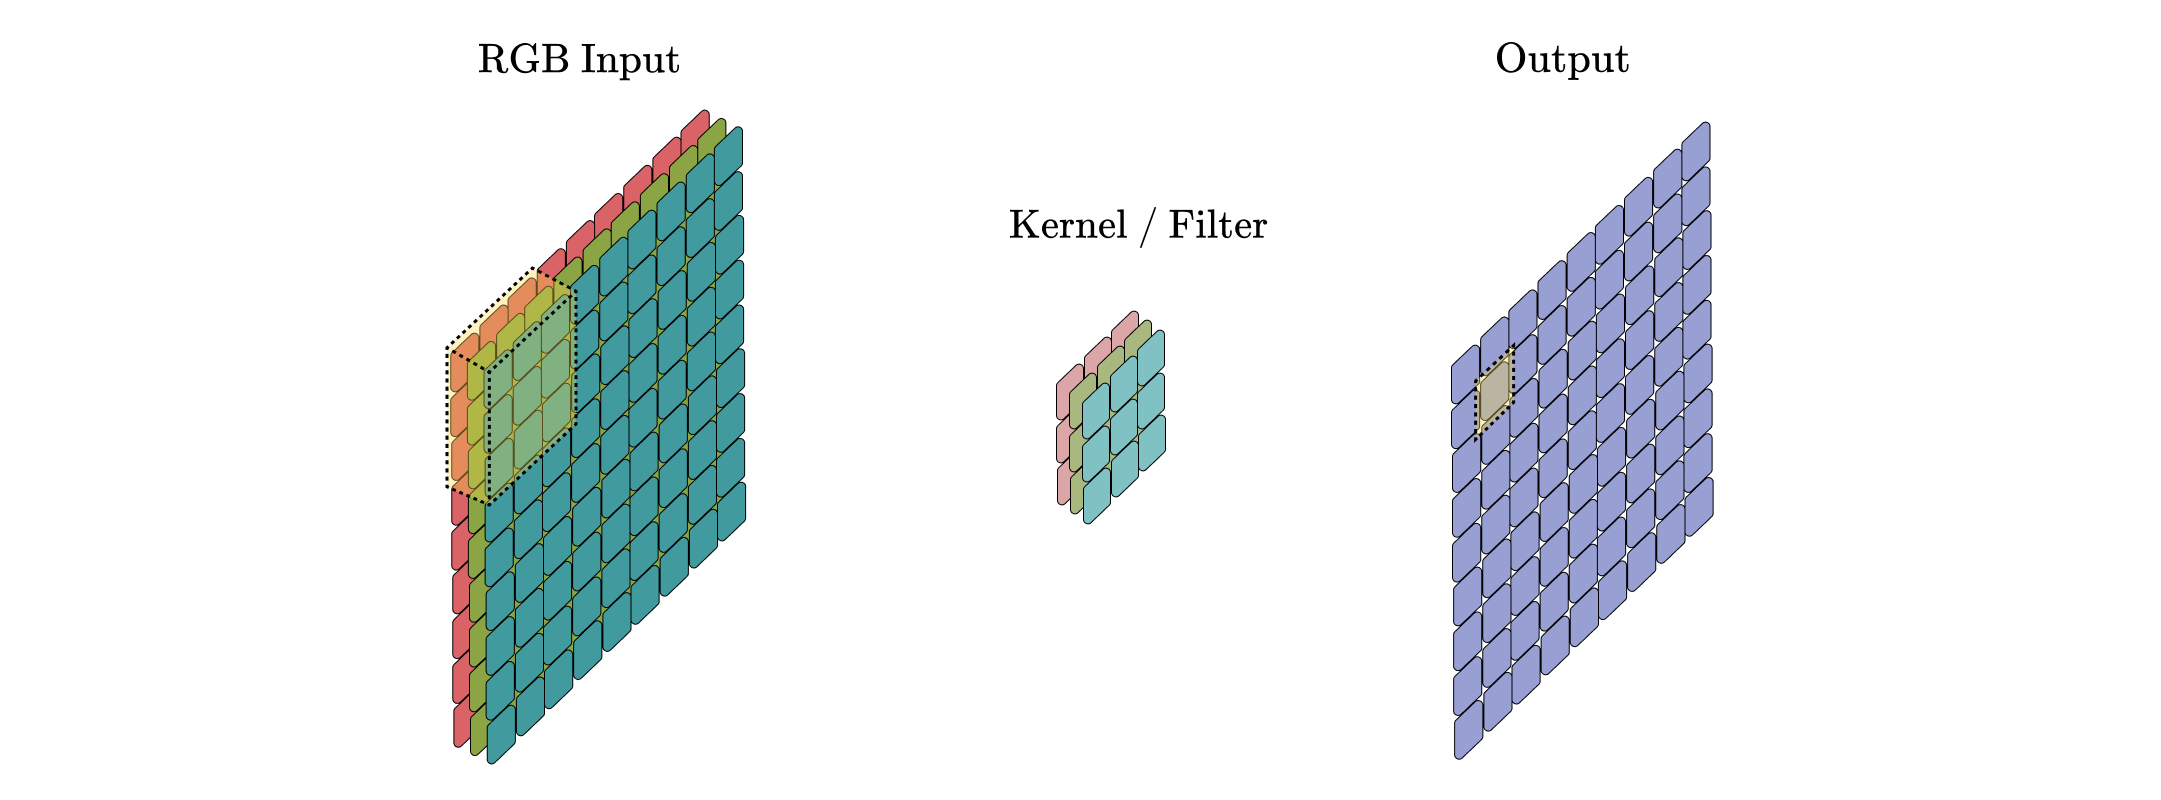
\includegraphics[width=14cm]{convolution_multiple_channels.png}
  \caption{A 3×3×3 kernel (filter) sliding over an RGB input matrix to produce a single-channeled output feature map.}
  \label{fig:convolution_multiple_channels}
\end{figure}
Mathematically, a convolutional layer can be represented as:
\[
y_{i,j,k} = f \left( \sum_{m=1}^c \sum_{p=1}^h \sum_{q=1}^w x_{i+p-1, j+q-1, m} \cdot w_{p,q,m,k} + b_k \right)
\]

\begin{itemize}
  \item \( h, w \) are the height and width of the filter, respectively.
  \item \( c \) is the number of input channels.
  \item \( y_{i,j,k} \) denotes the output at position \((i, j)\) for the \(k\)-th filter.
  \item \( x_{i+p-1, j+q-1, m} \) is the input at position \((i+p-1, j+q-1)\) for the \(m\)-th input channel.
  \item \( w_{p,q,m,k} \) is the weight of the \(k\)-th filter at \((p, q)\) for input channel \(m\).
  \item \( b_k \) is the bias for the \(k\)-th filter.
  \item \( f(\cdot): \mathbb{R} \to \mathbb{R} \) is the activation function.
\end{itemize}

In other words, a convolutional layer applies filter weights 
as it slides over rows \((p)\), columns \((q)\), and channels \((m)\), 
sums the results, adds bias \((b_k)\), 
and repeats this for all positions \((i, j)\) and filters \((k)\).

Although convolutional layers often have fewer weight parameters than dense layers in typical architectures, 
they still contain redundancies \cite{huang2017densely}, presenting an opportunity for quantization. 
Together, dense and convolutional layers form the building blocks of convolutional neural networks (CNNs), 
the core of breakthroughs in computer vision \cite{DBLP:journals/nature/LeCunBH15, DBLP:conf/nips/KrizhevskySH12, DBLP:conf/cvpr/SzegedyLJSRAEVR15}.
Thus, both dense and convolutional layers will be the focus of this work.

% -------------------- lossregularization --------------------


\subsection{Loss Functions and Regularization}
\label{subsec:lossregularization}
\hspace*{1em}The weights and biases of NN layers are usually \textit{learnable parameters}
that the model adjusts during \textit{training}.
The training process of NNs is similar to how our brains learn from mistakes. 
Given the ground truth, an NN adjusts its learnable parameters 
using a specific function that compares the ground truth with the output generated by the network, 
essentially measuring the magnitude of the network's errors.

This function is called a \textit{loss function}, and depending on the type of question the network aims to answer, it can take many different forms.
For example, for the MLP described in \cref{fig:dense_layer} that generates a binary classification, we would use the \textit{log loss} function. 
Since the datasets used in this thesis involve multi-class classification, the \textit{sparse categorical cross-entropy} (SCCE) loss function will be used, 
which measures the difference between the predicted class probabilities and the true labels for each class.

The loss function alone cannot ensure a neural network generalizes well to unseen data, 
as it focuses solely on minimizing error on the training set,
which can lead to overfitting or a failure to capture the desired generalization properties.
To mitigate overfitting,
a \textit{regularization term} is added to the loss function
to penalize unwanted behaviors.

A typical regularization term is \( L_2 \), 
which penalizes large weights by adding the sum of the squared weights to the loss. 
The modified loss function is then expressed as:
\[
\mathcal{L}_{\text{total}} = \mathcal{L}_{\text{task}} + \lambda \sum_{i} w_i^2
\]
\begin{itemize}
  \item \( \mathcal{L}_{\text{task}} \) is the original task-specific loss function (in our case, the SCCE loss function).
  \item \( \lambda \) is a scalar parameter that controls the strength of the regularization.
  \item \( w_i \) represents each individual weight value in the model.
\end{itemize}

Regularization terms may have different objectives, be it for better generalization, 
improved robustness, or encouraging sparsity in the model parameters. 
The current work employs multiple custom regularization terms 
that encourage quantization that we will discuss in detail in \cref{sec:customloss}.

% -------------------- forwardback --------------------

\subsection{Forward-Pass and Back-Propagation}
\label{subsec:forwardback}
\hspace*{1em} The repetition of the mathematical operations described earlier in \cref{subsec:denseconvolutional} 
during model training constitutes the \textit{forward pass}, 
the process where input data is passed through the network layer by layer, 
with each layer applying its learned weights and biases to produce a final output. 
This output is then compared with the ground truth by the loss function that produces an error
as explained in \cref{subsec:lossregularization}.
The error is then used to update the parameters in \textit{W} and \textit{b} during a process called \textit{back-propagation}.
In other words, back-propagation is the method by which the network adjusts its parameters to minimize the error. 
This method calculates the gradient of the loss function with respect to each parameter using the chain rule. 
\( W \) and \( b \) are updated as follows:
\[
W = W - \eta \frac{\partial L}{\partial W}, \quad b = b - \eta \frac{\partial L}{\partial b}
\]
where \( L \) is the loss function, and \( \eta \) is the learning rate.

For example, consider the weight \( w_{1,1} \) represented as the line between \( x_1 \)
 and the hidden layer node \( {a_1}^{(1)} \) in \cref{fig:dense_layer}. 
The gradient of this weight with respect to the loss is calculated using the chain rule,
as shown below:
\[
\frac{\partial L}{\partial w_{1,1}} = \frac{\partial L}{\partial o_1} \cdot \frac{\partial o_1}{\partial {a_1}^{(1)}} \cdot \frac{\partial {a_1}^{(1)}}{\partial w_{1,1}}
\]
\begin{itemize}
    \item \( \frac{\partial L}{\partial o_1} \) is the gradient of the loss with respect to \( o_1 \).
    \item \( \frac{\partial o_1}{\partial {a_1}^{(1)}} \) is the gradient of \( o_1 \) with respect to the output of \( {a_1}^{(1)} \).
    \item \( \frac{\partial {a_1}^{(1)} }{\partial w_{1,1}} \) is the value of  \( x_1 \), since  \( {a_1}^{(1)} \) is a weighted sum of the inputs.
\end{itemize}

The chain rule, and consequently backpropagation, is a critical bottleneck for quantization. 
This issue, along with its solution, will be detailed in \cref{sec:learnedquantization}.

% ------------------------------------------------------------
% ----------------------- basicsofquantization ----------------------- 
% ------------------------------------------------------------

\section{Basics of Quantization}
\label{sec:basicsofquantization}
\hspace*{1em}This section aims to motivate the use of quantization  
and further provides a broader understanding of the term regarding its types.

% -------------------- purpose and definition --------------------

\subsection{Purpose and Definition}
\label{subsec:purposeanddefinition}
\hspace*{1em}As we become increasingly dependent on deep learning models disguised as everyday tools, 
the need for these models to function in a resource- and time-efficient manner is more imperative than ever. 
The focus on resource efficiency is particularly important, 
with the research community expressing concerns regarding the environmental effects of large models, 
the exponential size growth of which continues to significantly outpace that of system hardware \cite{DBLP:journals/corr/abs-2111-00364}. 
In this regard, studies have examined quantization within the context of Green AI as a method to reduce the carbon footprint of
ML models \cite{DBLP:journals/csi/RegueroMV25}.

Aside from the environmental considerations, the mere need to reduce 
the computational cost and speed of predictive models
comes as an apparent business requirement. 
This requirement is essential when — quite ironically — embedded systems, famous for their compactness, meet 
ML models, recognized for their complexity. Microcontrollers, for instance, 
usually are not able to perform floating-point operations, which must therefore be emulated in software, 
introducing significant overhead. 
For this reason, quantization,
the process which reduces the memory footprint of a model,
is also extensively covered in the realm of embedded systems that 
inherently prefer integer arithmetic, as well as bitwise operations \cite{rastegari2016xnor, DBLP:conf/eccv/ZhangYYH18, DBLP:conf/codit/KhalifaM24, DBLP:journals/corr/abs-2105-13331}.

Another motivation for quantization — although somewhat controversial — is the fact that reducing the bit width of
ML models makes them robust to adversial attacks in certain cases \cite{DBLP:journals/corr/abs-2404-05639}.
This holds significant value in fields, such as autonomous driving,
where model vulnerability may result in fatal outcomes.
Interestingly enough, the use cases where such robustness is required also demand fast inference, 
as they rely on real-time predictions. Consider healthcare diagnostics needed for emergency scenarios 
or military defense mechanisms designed for immediate action.

The reasons for employing quantization are numeruous and varied, but regardless of the motivation,
the essence of the term itself — rooted in the early 20th century — remains unchanged:
quantization refers to the division of a quantity into a discrete number
of small parts \cite{gray1998quantization}. With regard to ML models, 
quantization describes the process of dividing higher bit-width numbers into a discrete number of lower bit-width representations
without causing significant degradation in accuracy \cite{gholami2021survey}.

Since ML models are generally considered redundant or over-parameterized,
there are multiple points where quantization can be applied.
Specifically, we apply quantization to the weights and biases of dense layers, 
as well as the kernels and biases of convolutional layers. 
Other applications include, but are not limited to, layer activation and layer input quantization (two sides of the same coin),
as well as gradient quantization. The bottom line is that wherever there is an opportunity for arithmetic or memory optimization,
there is room for quantization.

% -------------------- Common Quantization Approaches --------------------

\subsection{Core Quantization Approaches}
\label{subsec:commonquantizationapproaches}
\hspace*{1em}There is a multitude of ways to classify NN quantization methods, a broader overview of which will be covered
in \cref{cha:chapter5}.
For now, we will focus on a few basic approaches from the general categories of both 
\textit{data-driven} and \textit{data-free} methods \cite{Edouard2022SPIQ} to provide a basic understanding of the NN quantization process.

A basic form of data-free quantization, or \textit{post-training quantization} \cite{jiang2021efficient},
involves converting already trained parameters from FP32 to a lower bit-width format
without using the initial training data. 
One approach is to apply \textit{uniform quantization} that maps real values to a set number
of \textit{bins}. The formula can be written as:
\[
Q(r) = \left\lfloor \frac{r}{S} \right\rfloor
\]

\newpage
\begin{itemize}
    \item $Q(\cdot)$ denotes the quantization operation.
    \item $r$ is the real value of a given model parameter in higher bit-width representation.
    \item $S$ is a scaling factor.
\end{itemize}
As a result, we end up with values that can directly be cast to a lower bit-width representation,
forming a discrete set of bins instead of an almost continuous range of real numbers,
as shown in \cref{fig:quantizing_example}.
\begin{figure}[b!]
  \centering
  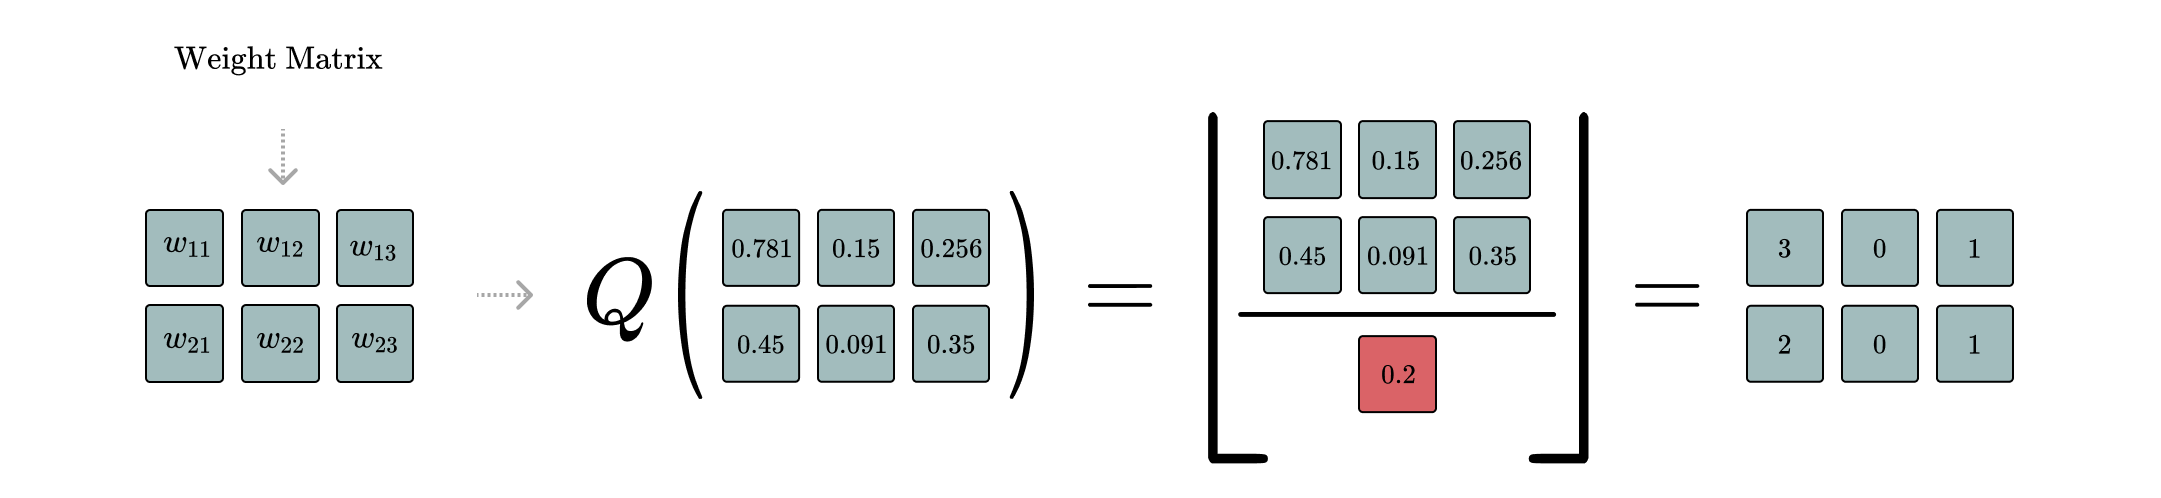
\includegraphics[width=14cm]{quantizing_example.png}
  \caption{Uniform quantization of an arbitrary weight matrix.}
  \label{fig:quantizing_example}
\end{figure}

Unlike data-free quantization  —  as the name suggests — data-driven quantization involves retraining the model
using the initial data. An example of this approach is the Ristretto framework \cite{DBLP:journals/tnn/GyselPMG18}, which, similar to data-free methods, 
first analyzes the trained model to select suitable lower bit-width number formats for its weights.
Then, using a portion of the original dataset, the framework determines appropriate formats for layer inputs and outputs.
As a next step, based on the validation data, Ristretto adjusts the quantization settings to achieve optimal performance 
under the given constraints. Finally, the quantized model is fine-tuned using the training data.

A basic example of data-driven quantization is min-max quantization on input data, as shown in Figure \ref{fig:min_max_quantization},
using the formula for 8-bit quantization:
\[
Q_{\textit{MinMax}}(x) = \left\lfloor \frac{x - \min(X)}{s} \right\rfloor, \quad
\text{where} \quad s = \frac{\max(X) - \min(X)}{2^8 - 1}
\]

This method can also be implemented in a data-free scenario to quantize learned model parameters and is internally used as one of the
default techniques in popular ML frameworks like Tensorflow and PyTorch. 

\begin{figure}[t!]
  \centering
  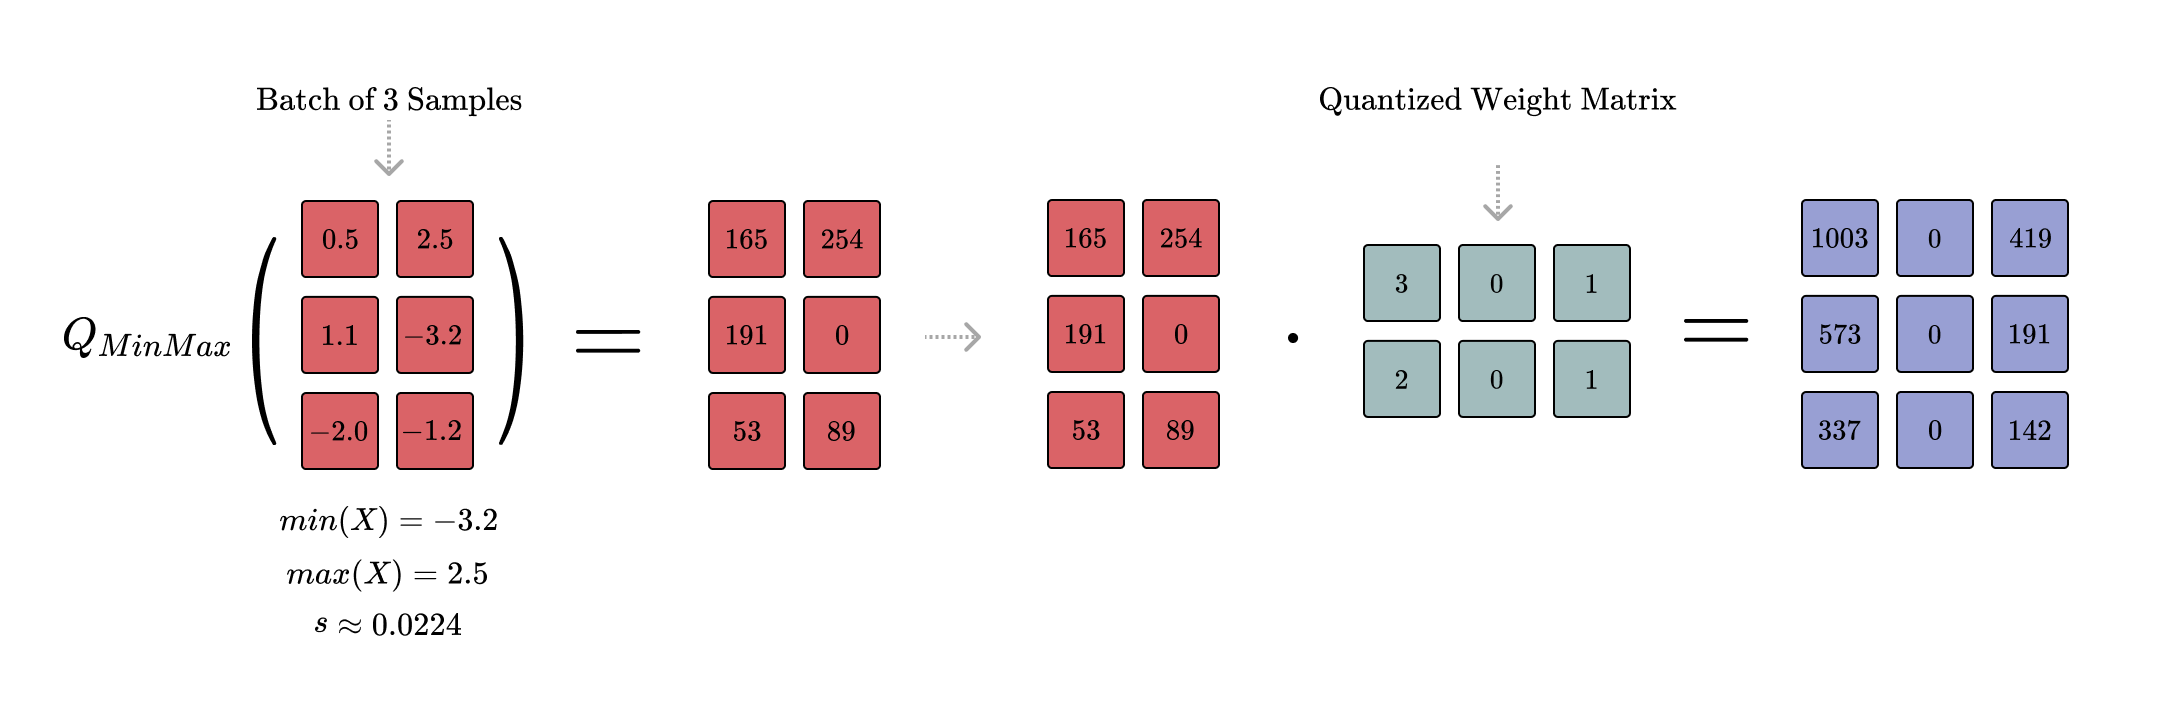
\includegraphics[width=14cm]{min_max_quantization.png}
  \caption{ Min-max quantization of input data to 8 bits, followed by matrix multiplication with the quantized weight matrix.}
  \label{fig:min_max_quantization}
\end{figure}

Previously, we discussed \textit{where} quantization could be applied in a model, 
mentioning weights, kernels, and biases as the focus of this thesis.
\cref{fig:quantizing_example} and \cref{fig:min_max_quantization} show examples of quantization
using a scalar scaling factor. 
However, scaling factors can be applied at varying levels of detail,
bringing forth the concept of \textit{quantization granularity}.

Granularity refers to the level of detail at which \textit{quantizers} — such as scaling factors, offset adjustments, or other binning strategies 
— are applied,
ranging from a single quantizer for an entire kernel (coarse granularity) to separate ones for individual spatial locations,
channels, or filters (fine granularity). 

\cref{fig:granularity-conv2d} illustrates various scaling factor granularities
for the kernels of convolutional layers.
Despite this wide range of possibilities, channel-wise quantization is currently the standard for convolutional layers \cite{gholami2021survey},
as it helps parallel processing capabilities of accelerators that compute channel outputs independently. 
For dense layers, row-wise quantization (one scaling factor for weights used by a single output neuron) is more prevalent
because it aligns with matrix-vector multiplication, which then can be carried out by specialized linear algebra libraries
in an optimized way \cite{DBLP:journals/corr/abs-2101-05615}.
Thus, in the experiments, we focus our quantization methods on channel-wise granularity for convolutional layers
and row-wise granularity for dense layers, 
while also exploring a few additional applications.

\begin{figure}[t!]
  \centering
  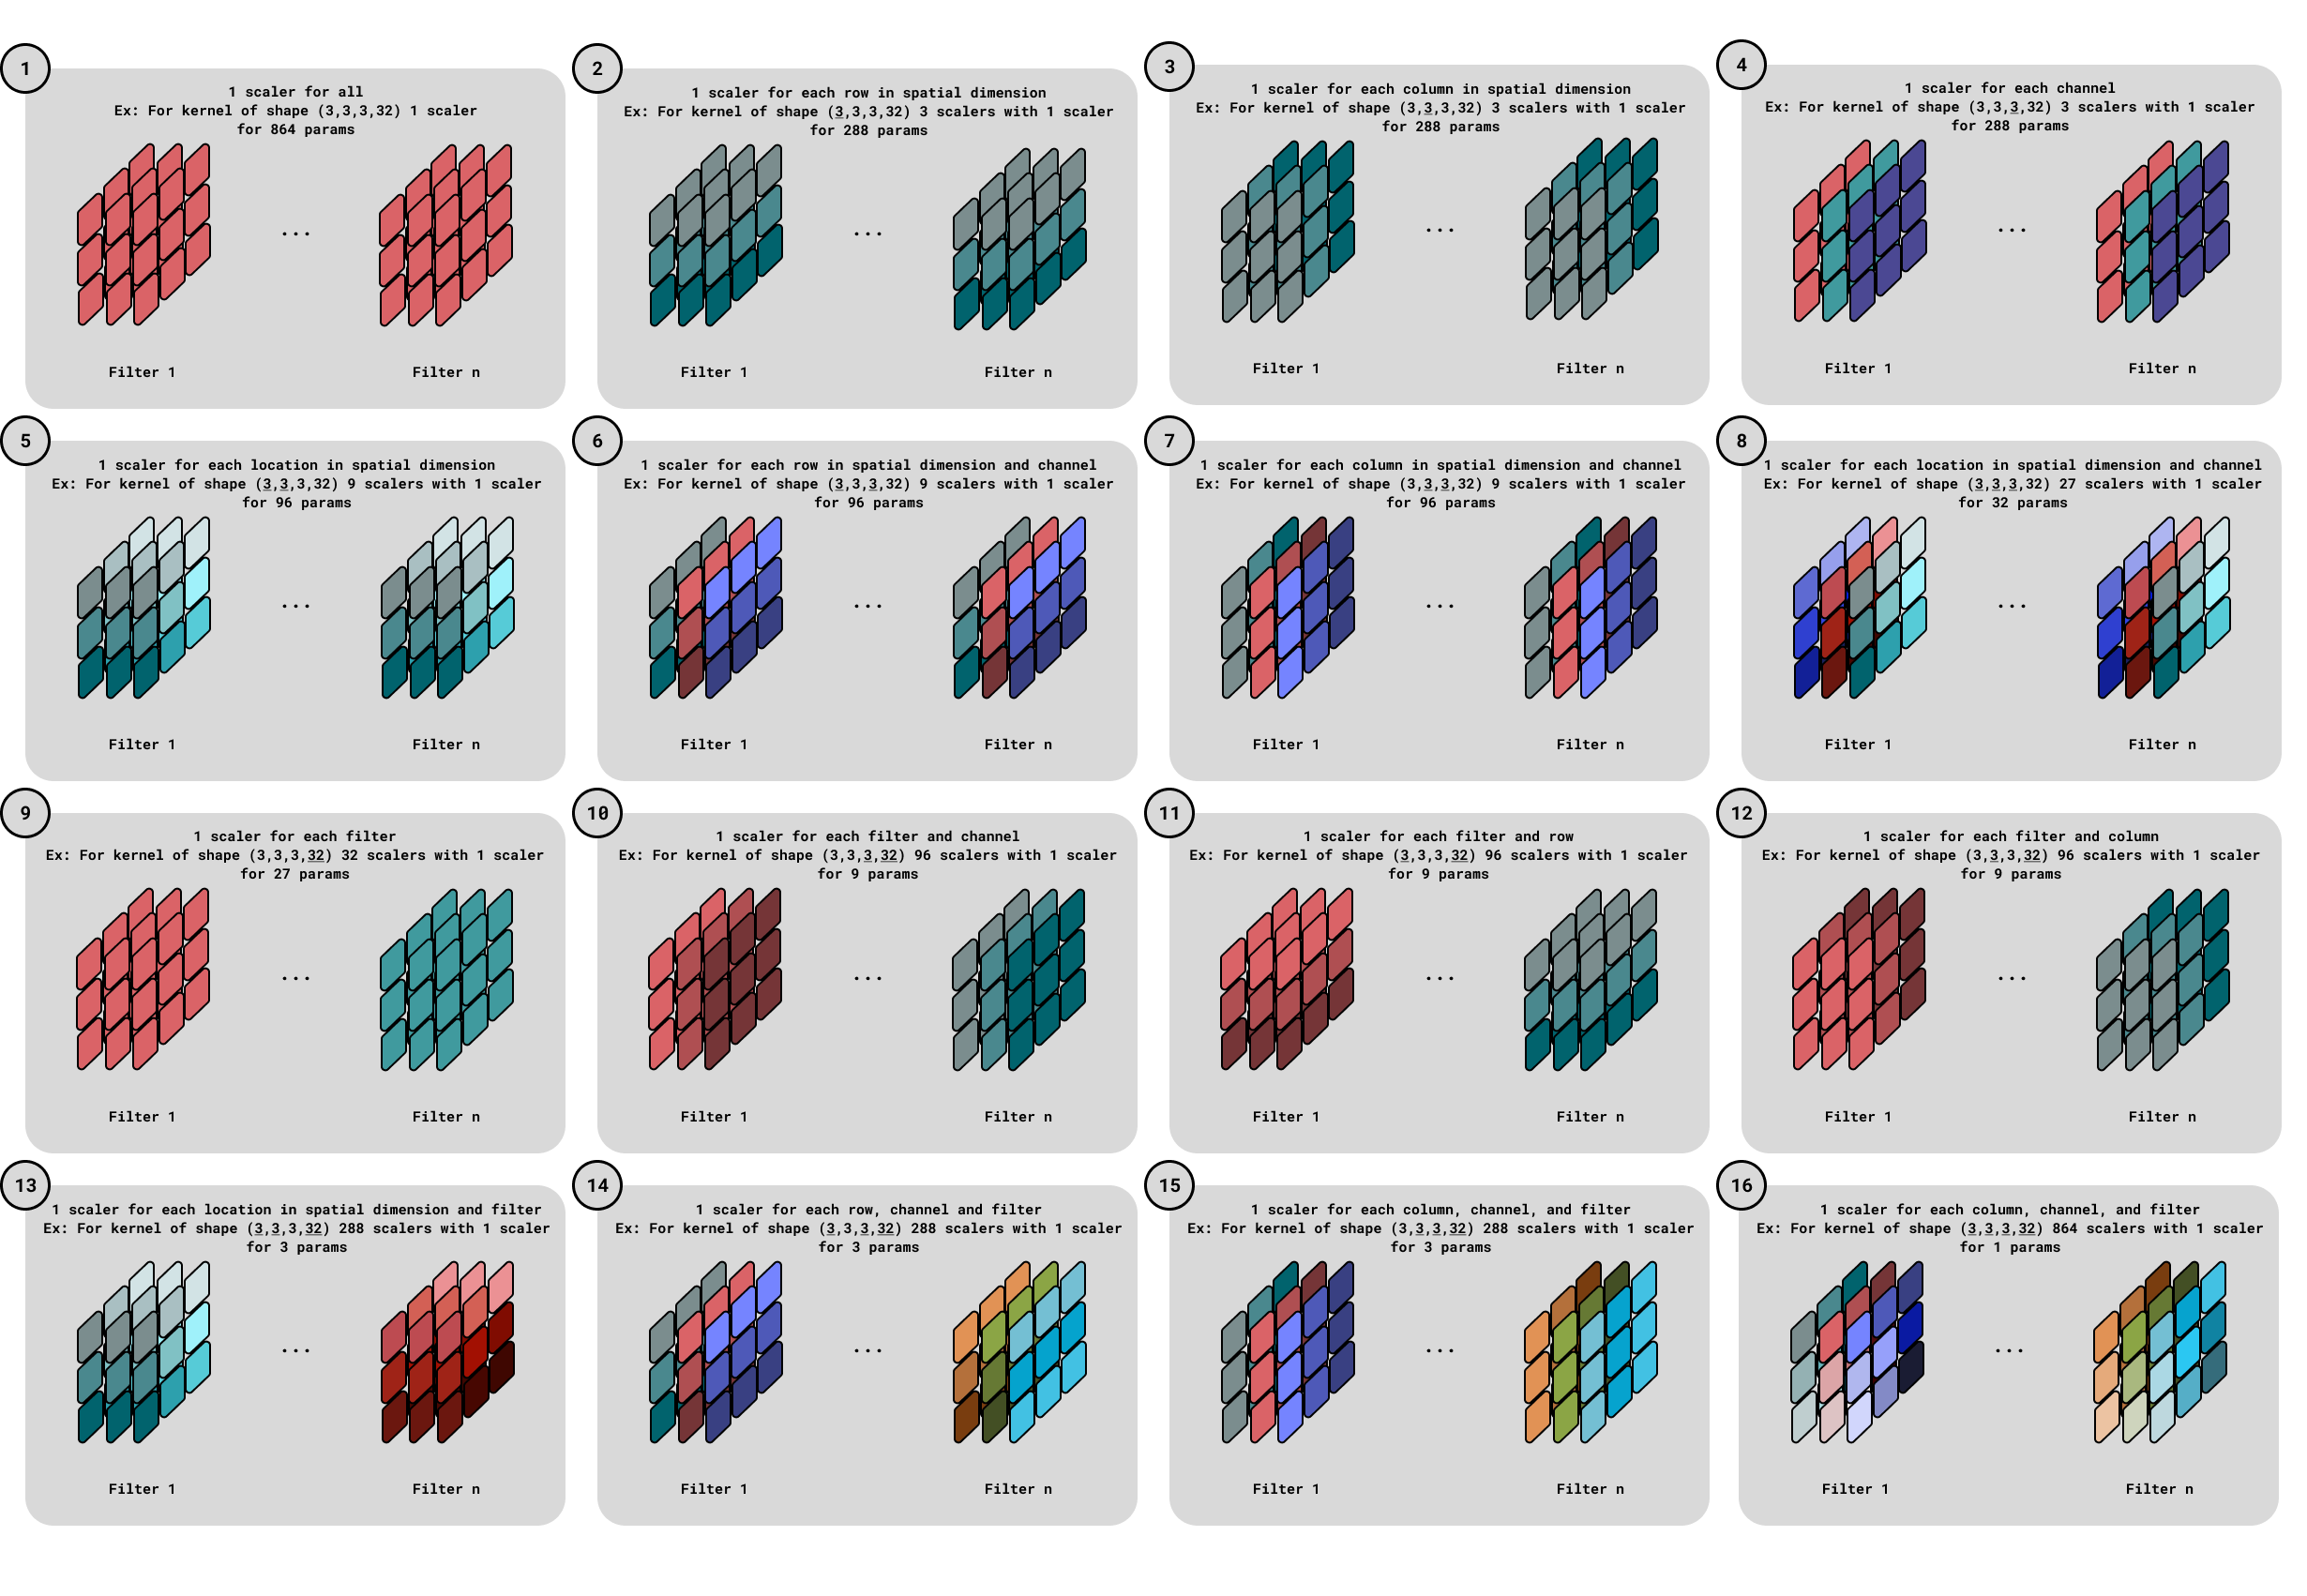
\includegraphics[width=14cm]{granularity-conv2d.png}
  \caption{Various applications of scaling factors, ranging from a single scalar applied to the entire kernel (1) to separate scalars assigned to spatial dimensions (e.g., 1, 2), channels (4), filters (9), and other granular configurations.}
  \label{fig:granularity-conv2d}
\end{figure}



% ------------------------------------------------------------
% ----------------------- learnedquantization ----------------------- 
% ------------------------------------------------------------
\section{Learned Quantization}
\label{sec:learnedquantization}
\hspace*{1em}Now that the fundamentals of quantization have been covered, 
this section introduces key concepts commonly encountered in learned quantization,
including its challenges, trade-offs, and the popular techniques used to overcome them.


% -------------------- tradeoffs and challenges --------------------

\subsection{Trade-offs and Challenges}
\label{subsec:subsection1}
\hspace*{1em}The inherent — or rather the widely accepted — characteristic of quantization is
that it negatively influences accuracy. 
The trade-off between quantization and generalization 
refers to the balance of how much accuracy we are willing to sacrifice
 to gain a reduction in computational cost, memory usage, or inference time.
However, the truth is that we usually cannot afford sacrificing anything. 
This challenge, coupled with the lack of a guarantee
 that predefined quantizers can yield optimal results \cite{DBLP:conf/eccv/ZhangYYH18, DBLP:conf/iclr/EsserMBAM20}, 
 has paved the way for the burgeoning field of learned quantization,
 which aims to \textit{learn} how to quantize the model in a manner that mitigates performance loss.

Learned quantization is, however, a double-edged sword in the sense that, despite producing compact results,
the cost to achieve them is higher \cite{DBLP:conf/eccv/ParkYV18}. The obvious reason is the additional computational overhead
introduced by learnable quantizers.
Thus, it is important to strike a balance between learning optimal quantization and keeping the training process manageable
— which explains the prevailing emphasis on simplicity in most learned quantization research.

The main issue in achieving this simplicity is posed by the fact that discretization, in its essence, is non-differentiable
 — meaning it is challenging to integrate any kind of discretizing operations into gradient-based optimization methods, 
 upon which ML models rely. Using the chain rule back-propagation example from \cref{subsec:forwardback}, let us
consider a simple flooring operation introduced into the process to better understand the problem.
Suppose we quantize activations and apply \( \lfloor \cdot \rfloor \) to hidden layer outputs:
\[
  {a_{1,q}}^{(1)} =  \lfloor {a_1}^{(1)} \rfloor
  \]
As a result, the chain rule becomes:
 \[
  \frac{\partial L}{\partial w_{1,1}} =  \frac{\partial L}{\partial {a_{1,q}}^{(1)}} 
  \cdot \frac{\partial {a_{1,q}}^{(1)}}{\partial {a_1}^{(1)}} 
  \cdot \frac{\partial {a_1}^{(1)}}{\partial w_{1,1}}
  \]
where \( \frac{\partial {a_{1,q}}^{(1)}}{\partial {a_1}^{(1)}} \) presents a challenge. 
  Since \(  {a_{1,q}}^{(1)} =  \lfloor {a_1}^{(1)} \rfloor \), the derivative is: 
            \[
            \frac{\partial a_{1,q}^{(1)}}{\partial a_{1}^{(1)}} =
            \begin{cases} 
                0 & \text{if } a_{1}^{(1)} \notin \mathbb{Z}, \\
                \text{undefined} & \text{if } a_{1}^{(1)} \in \mathbb{Z}.
            \end{cases}
            \]

This means that for most values of \( {a_1}^{(1)} \), which are non-integer, the gradient becomes $0$, resulting in 
  $w_{1,1}$ not receiving any updates. For integer values of \( {a_1}^{(1)} \), the back-propagation process fails altogether.

In essence, circumventing the issue of non-differentiability is the fundamental problem that learned quantization aims to solve,
all while managing the aforementioned trade-offs to produce a model that is compact, not overly complex to train,
and highly performant.

% -------------------- common methods --------------------

\subsection{Common Methods}
\label{subsec:commonlearnedquantizationmethods}

\hspace*{1em}The most common method to address the issue of non-differentibility is to approximate the gradient of quantization operators
using the Straight-Through Estimator (STE) \cite{bengio2013estimating, fan2021training, DBLP:conf/eccv/ZhangYYH18}. 
This workaround applies the quantization operation \textit{as is} 
during the forward-pass, but replaces the gradient of the piece-wise discontinuous function 
with that of a continuous identity function. Returning to the example from the previous subsection,
if we apply the STE to the problematic gradient, instead of:
\[
  \frac{\partial a_{1,q}^{(1)}}{\partial a_{1}^{(1)}} =
  \begin{cases} 
      0 & \text{if } a_{1}^{(1)} \notin \mathbb{Z}, \\
      \text{undefined} & \text{if } a_{1}^{(1)} \in \mathbb{Z}.
  \end{cases}
  \]
we approximate it as: 
\[
  \frac{\partial a_{1,q}^{(1)}}{\partial a_{1}^{(1)}}  \approx 1
  \]
This approximation enables gradient flow, allowing model parameters to receive updates
without being hindered by the non-differentiability of the quantization step.

The STE — and other estimators \cite{DBLP:journals/jstsp/Chen0ZHY20} —  are the cornerstone of quantization-aware training (QAT) \cite{jacob2018quantization},
a subfield that falls under the broader umbrella of learned quantization.
QAT, however, does not necessarily focus on learning quantization parameters.
Instead, it focuses on helping the model adapt to the loss caused by the quantization process during the forward pass,
whether or not trainable quantizers are involved.

More often than not QAT and trainable quantization parameters are combined. 
An example is quantization-interval-learning (QIL) \cite{DBLP:conf/cvpr/JungSLSHKHC19}, 
which uses three trainable quantization parameters 
(the center of the interval, the distance to the center, and a parameter that controls the scaling itself) 
with piecewise differentiable operations and relies on STE for gradient updates of quantized weights and activations. 
Similarly, the learned step size quantization (LSQ) approach \cite{DBLP:conf/iclr/EsserMBAM20} 
defines a single trainable quantization parameter (step size) with an explicit gradient formula and also uses STE for standard parameter updates.
LQ-Nets \cite{DBLP:conf/eccv/ZhangYYH18} depend on STE too, but  —  unlike the two previous techniques — 
directly incorporate a quantization error minimization algorithm to calculate binary encodings and the associated bases of
model parameters given a predefined bit size. 

Another way to achieve learned quantization is through the use of a regularization term. 
Such regularization terms are often periodic functions, 
such as sinusoidal functions \cite{DBLP:journals/corr/abs-1811-09862,DBLP:journals/corr/abs-1905-01416}, 
which pull model parameters toward the nearest step — or quantization bin.
A notable example is WaveQ \cite{DBLP:journals/corr/abs-2003-00146},
which combines a sine regularizer with an additional term that encourages lower bit widths
without predefined bit constraints. A more straight-forward regularizer is
the Mean Squared Quantization Error \cite{DBLP:journals/access/ChoiEL20}
that directly minimizes the difference between the high-precision parameters
and their quantized counterparts.

In this thesis, we will utilize STE but introduce a custom gradient calculation for the scale factor gradients
based on a specific type of gradient sensitivity in the model parameters.
Additionally, we will explore custom loss regularization terms that encourage quantization
and systematically compare them across different datasets.